%&<latex>
\documentclass[12pt]{article}
\pagestyle{plain}
\usepackage{anysize}
\papersize{11in}{8.5in}
\marginsize{1in}{1in}{.5in}{.5in}
\pagenumbering{arabic}
\usepackage{setspace}
\usepackage[usenames]{color}
\usepackage[fleqn]{amsmath}
\usepackage{amssymb}
\usepackage{graphicx}
\usepackage{indentfirst}
\usepackage{ragged2e}
\usepackage{upgreek}
\usepackage{xspace}
\usepackage{ifthen}
\usepackage{parskip}
\usepackage[normalem]{ulem}
\usepackage[round]{natbib}
\bibliographystyle{evolution}
\usepackage{hyperref}
\hypersetup{pdfborder={0 0 0}, colorlinks=true, urlcolor=blue, linkcolor=blue, citecolor=blue}
\usepackage{tikz}
\usetikzlibrary{arrows}

\newcommand{\myIfArg}[2]{\ifthenelse{\equal{#1}{}}{}{#2}}

\newcounter{revCommentCounter}[section]
\setcounter{revCommentCounter}{0}
\numberwithin{revCommentCounter}{section}
\renewcommand{\thesubsection}{\Alph{subsection}}

\newcommand{\revcomment}[6]{\refstepcounter{revCommentCounter}%
    \medskip \hrule \noindent%
    \textbf{\therevCommentCounter}:
    \myIfArg{#1}{#1, }%
    \myIfArg{#2}{Page #2, }%
    \myIfArg{#3}{Column #3, }%
    \myIfArg{#4}{Paragraph #4, }%
    \myIfArg{#5}{Line #5}%
    \par\addtolength{\leftskip}{0.25in}%
    #6\par\addtolength{\leftskip}{-0.25in}\xspace}

\providecommand{\e}[1]{\ensuremath{\times 10^{#1}}}
\newcommand{\ifTwoArgs}[3]{\ifthenelse{\equal{#1}{}\or\equal{#2}{}}{}{#3}\xspace}
\newcommand{\ifArg}[2]{\ifthenelse{\equal{#1}{}}{}{#2}\xspace}
\newcommand{\msb}{\upshape\texttt{msBayes}\xspace}
\newcommand{\meant}[2]{\ensuremath{E(\divt{#1})_{#2}}}
\newcommand{\vmratio}[1]{\ensuremath{\Omega_{#1}}}
\newcommand{\numt}[1]{\ensuremath{\Psi_{#1}}}
\newcommand{\divt}[1]{\ensuremath{\tau_{#1}}}
\newcommand{\ssVector}[1]{\ensuremath{\mathbf{\alignmentSS{#1}{}}}\xspace}
\newcommand{\ssVectorObs}{\ensuremath{\ssVector{}^*}\xspace}
\newcommand{\alignmentSS}[2]{\ensuremath{S_{#1\protect\ifTwoArgs{#1}{#2}{,}#2}}\xspace}
\newcommand{\ssMatrix}{\ensuremath{\mathbb \alignmentSS{}{}}\xspace}

\let\quoteOld\quote
\let\endquoteOld\endquote
\renewenvironment{quote}{\sffamily\slshape\small\quoteOld}{\endquoteOld}

\makeatletter
\renewcommand{\section}{\@startsection{section}{1}{0mm}%
    {-8pt}%
    {4pt}%
{\sffamily\large\itshape}}
\makeatother

\tikzset{
  treenode/.style = {align=center, inner sep=0pt, text centered,
    font=\sffamily},
  tipnode/.style = {treenode, circle, white, font=\sffamily\bfseries, draw=black,
    fill=black, text width=1.5em},
  intnode/.style = {treenode, circle, draw=black, fill=black,
    minimum width=0.5em, minimum height=0.5em},
  arn_n/.style = {treenode, circle, white, font=\sffamily\bfseries, draw=black,
    fill=black, text width=1.5em},% arbre rouge noir, noeud noir
  arn_r/.style = {treenode, circle, red, draw=red, 
    text width=1.5em, very thick},% arbre rouge noir, noeud rouge
  arn_x/.style = {treenode, rectangle, draw=black,
    minimum width=0.5em, minimum height=0.5em}% arbre rouge noir, nil
}

\tikzstyle{centered} = [align=center, text centered, font=\sffamily\bfseries]
% \tikzstyle{skip} = [inner sep=0pt,fill]
\tikzstyle{skip} = [centered, inner sep=0pt, fill]
\tikzstyle{inode} = [centered, circle, minimum width=4pt, fill=black, inner sep=0pt]
\tikzstyle{tnode} = [centered, circle, inner sep=1pt]
% \tikzstyle{level 1}=[level distance=3.5cm, sibling distance=2cm]


\begin{document}

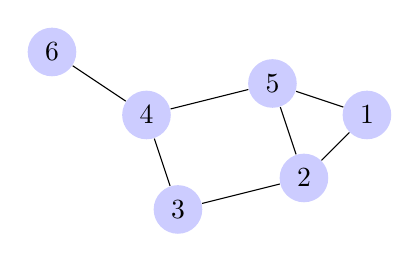
\begin{tikzpicture}
  [scale=0.4,auto=left,every node/.style={circle,fill=blue!20}]
  \node (n6) at (1,10) {6};
  \node (n4) at (4,8)  {4};
  \node (n5) at (8,9)  {5};
  \node (n1) at (11,8) {1};
  \node (n2) at (9,6)  {2};
  \node (n3) at (5,5)  {3};

  \foreach \from/\to in {n6/n4,n4/n5,n5/n1,n1/n2,n2/n5,n2/n3,n3/n4}
    \draw (\from) -- (\to);

\end{tikzpicture}

Below are three phylogenetic trees showing the relationships of
species A, B, C, and D. Which trees show the same relationships?\\
\begin{description}
    \item[A.] Tree 1 and 2.
    \item[B.] Tree 1 and 3.
    \item[C.] Tree 2 and 3.
    \item[D.] All.
    \item[E.] None.
\end{description}

\begin{tikzpicture}
[scale=0.7,auto=left,every node/.style={circle}]%,fill=blue!20}]
  \node [tnode](t1) at (1, 7) {A};
  \node [tnode](t2) at (3, 7) {B};
  \node [tnode](t3) at (5, 7) {C};
  \node [tnode](t4) at (7, 7) {D};
  \node [inode](i5) at (2, 5)  {};
  \node [skip](i6) at (4, 5)  {};
  \node [skip](i7) at (6, 5)  {};
  \node [inode](i8) at (3, 3)  {};
  \node [skip](i9) at (5, 3)  {};
  \node [inode, label=below: {\large\bf 1}](r) at (4, 1)  {};

  \foreach \from/\to in {r/i9,r/i8,i9/i7,i7/t4,i8/i5,i8/i6,i5/t1,i5/t2,i6/t3}
    \draw (\from) -- (\to);

  \node [tnode](t1) at (9, 7) {A};
  \node [tnode](t2) at (11, 7) {B};
  \node [tnode](t3) at (13, 7) {D};
  \node [tnode](t4) at (15, 7) {C};
  \node [inode](i5) at (10, 5)  {};
  \node [skip](i6) at (12, 5)  {};
  \node [skip](i7) at (14, 5)  {};
  \node [inode](i8) at (11, 3)  {};
  \node [skip](i9) at (13, 3)  {};
  \node [inode, label=below: {\large\bf 2}](r) at (12, 1)  {};

  \foreach \from/\to in {r/i9,r/i8,i9/i7,i7/t4,i8/i5,i8/i6,i5/t1,i5/t2,i6/t3}
    \draw (\from) -- (\to);

  \node [tnode](t1) at (17, 7) {C};
  \node [tnode](t2) at (19, 7) {B};
  \node [tnode](t3) at (21, 7) {A};
  \node [tnode](t4) at (23, 7) {D};
  \node [skip](i5) at (18, 5)  {};
  \node [inode](i6) at (20, 5)  {};
  \node [skip](i7) at (22, 5)  {};
  \node [inode](i8) at (19, 3)  {};
  \node [skip](i9) at (21, 3)  {};
  \node [inode, label=below: {\large\bf 3}](r) at  (20, 1)  {};

  \foreach \from/\to in {r/i9,r/i8,i9/i7,i7/t4,i8/i5,i8/i6,i5/t1,i6/t2,i6/t3}
    \draw (\from) -- (\to);


\end{tikzpicture}

% \begin{tikzpicture}[,>=stealth',grow=up,level/.style={sibling distance = 5cm/#1,
% \begin{tikzpicture}[,grow=up,level/.style={sibling distance = 5cm/#1,
%   level distance = 1.5cm}] 
% \node [arn_n] {33}
% child{ node [arn_r] {r}
%     child{ node [arn_r] {15} 
%             child{ node [arn_n] {10} 
%             	child{ node [arn_r] {5} edge from parent node[above left]
%                          {$x$}} %for a named pointer
% 							child{ node [arn_x] {}}
%             }
%             child{ node [arn_n] {20}
% 							child{ node [arn_r] {18}}
% 							child{ node [arn_x] {}}
%             }                            
%     }
%     child{ node [end] {}
%             child{ node [end] {} 
% 							child{ node [end] {}}
% 							child{ node [end] {}}
%             }
%             child{ node [end] {}
%                 child{ node [end, label=above: {A}] {}}
% 							child{ node [end] {}}
%             }
% 		}
%     }
% ; 
% \end{tikzpicture}

\end{document}

